\mode*


%%%%%%%%%%%%%%%%%%%%%%%%%%%%%%%%%%%%%%%%%%%%%%%%%%%%%%%%%%%%%%%%%%%%%%%%% 


\begin{frame}
  \frametitle{Fin de la loi de Moore ?}
  \begin{center}
    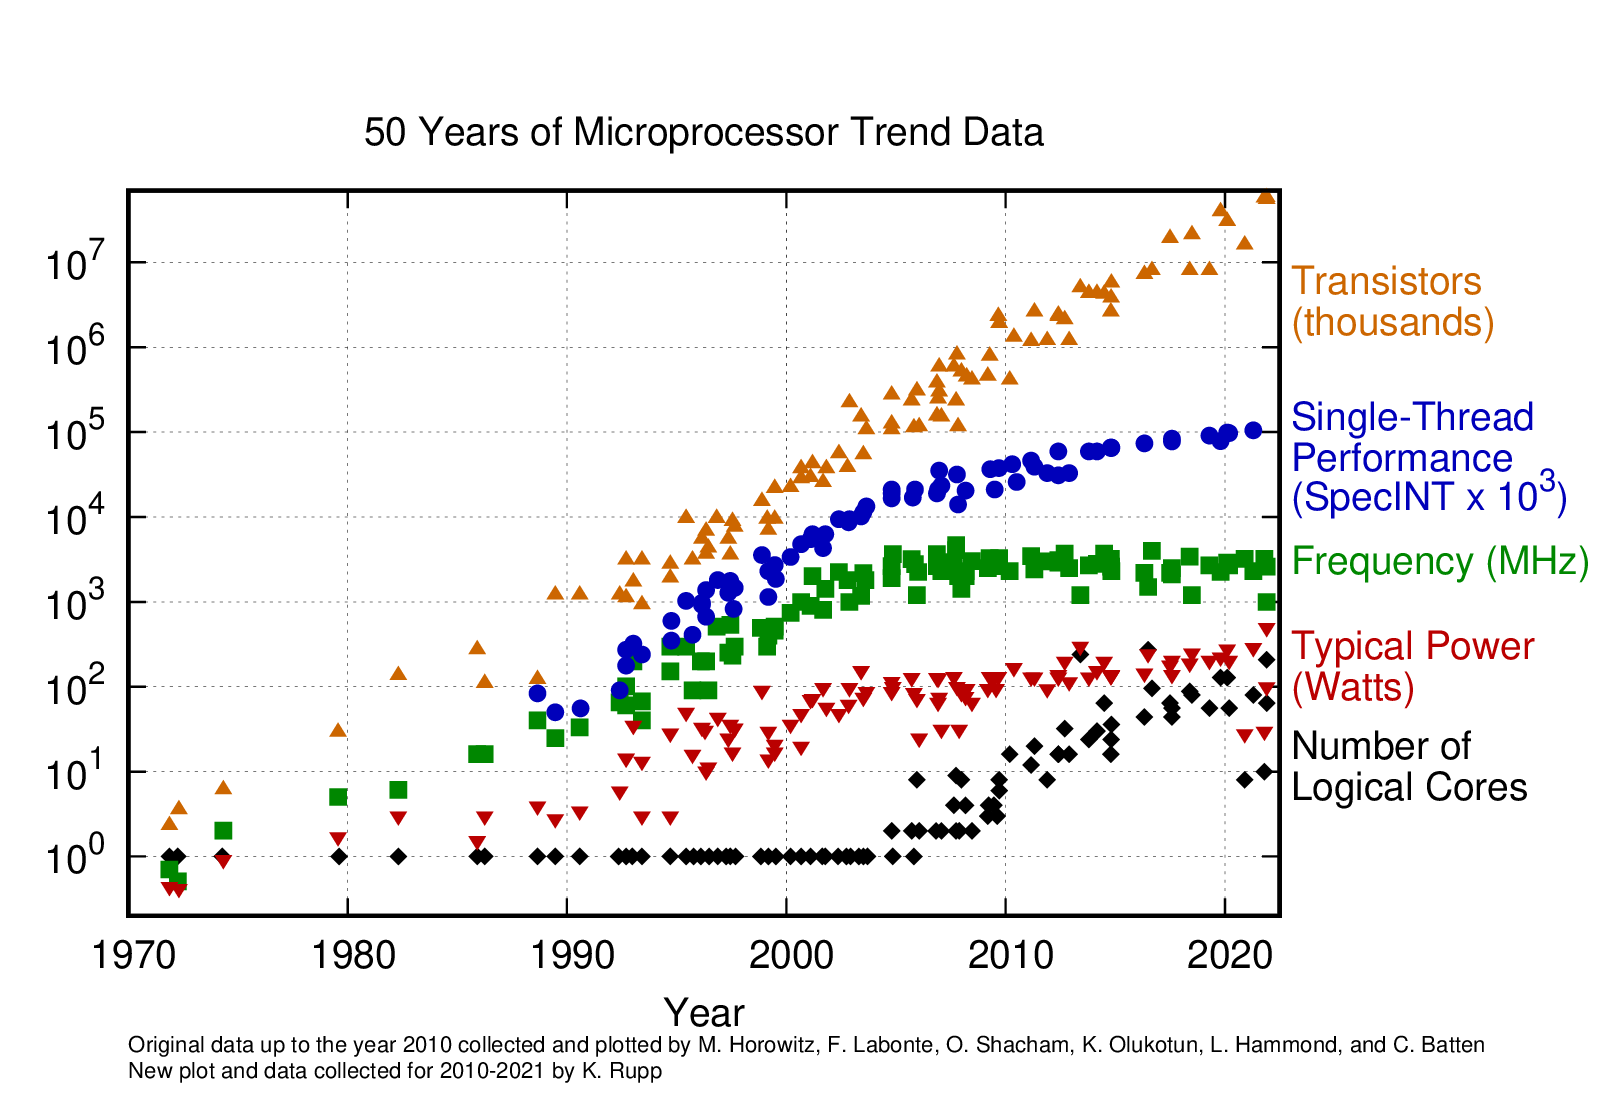
\includegraphics[width=.7\textwidth]{50-years-processor-trend.png}
    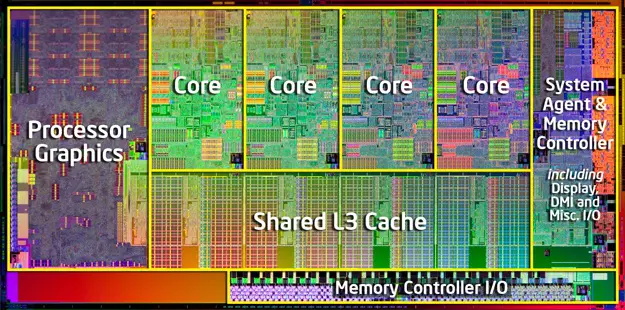
\includegraphics[width=.4\textwidth]{multic.png}
  \end{center}
\end{frame}


\begin{frame}{Buts de la programmation multi-c\oe urs}
   \begin{tikzpicture}[remember picture,overlay]
   \draw (5.5,2.2) node{\begin{minipage}{\textwidth}
      \begin{exampleblock}{Calculs coûteux}
         \begin{itemize}
         \item En temps de processeur (simulations scientifiques, \dots)
         \item<2-> En entrées/sorties (recherche dans les fichiers, \dots)
         \end{itemize}
      \end{exampleblock}
      \end{minipage}
   };

   \draw<1> (5.5,-1) node{
      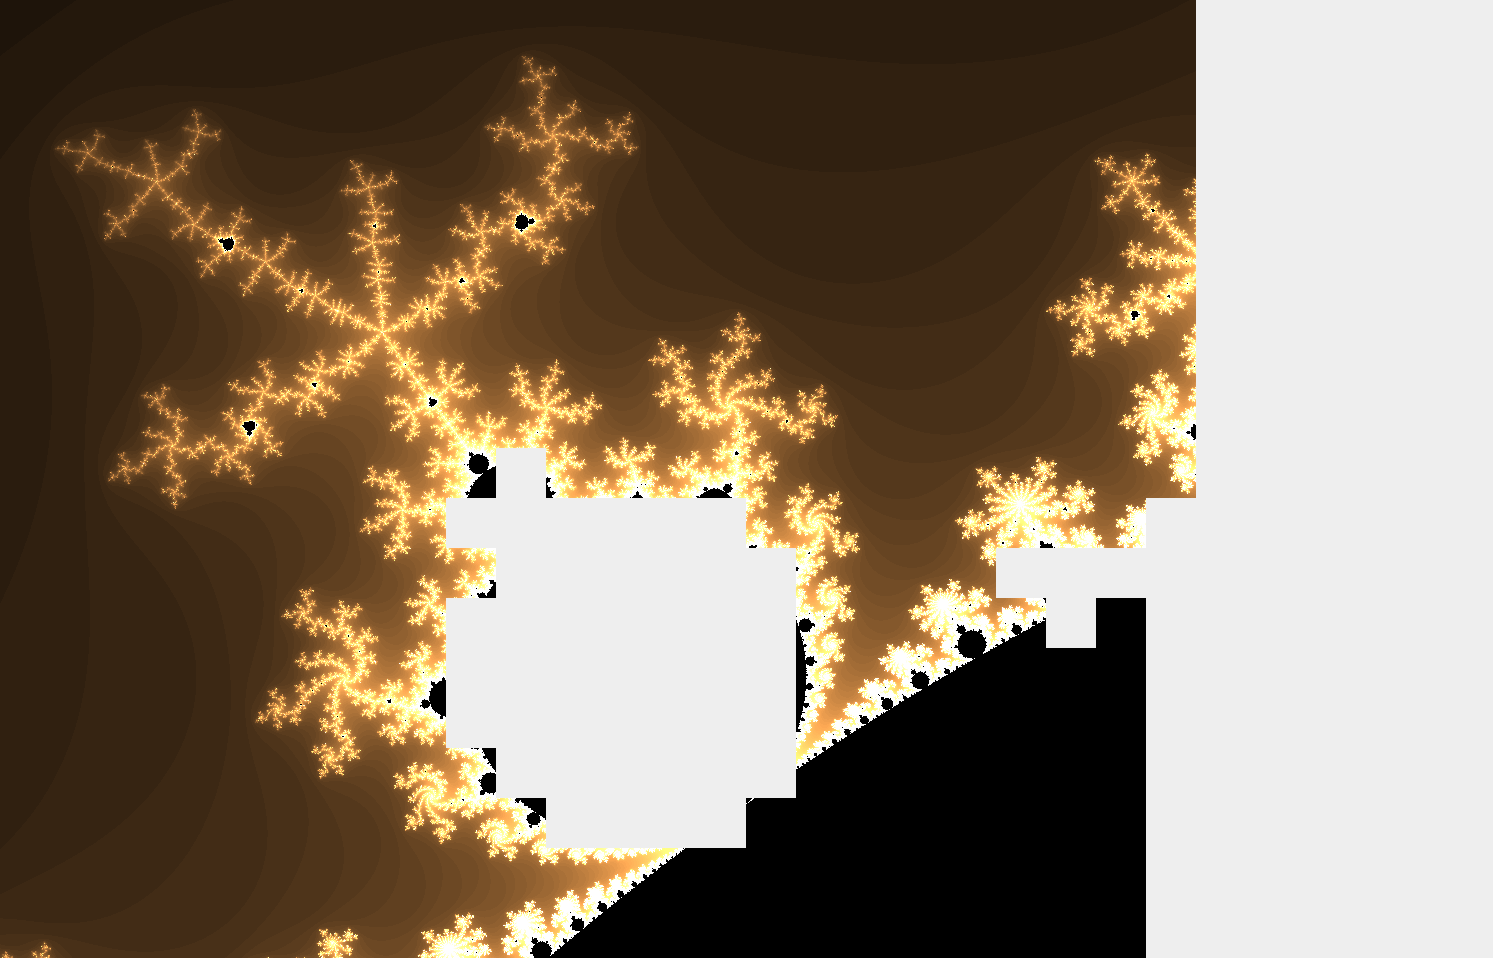
\includegraphics[height=.4\textwidth]{distanciel.png}
   };

   \draw<2> (5.5,-1) node{
        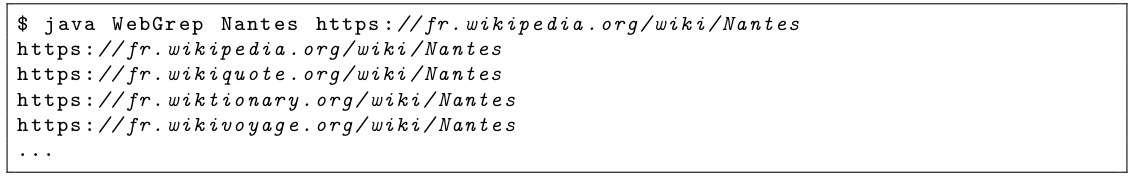
\includegraphics[width=.8\textwidth]{TP3.png}
   };

   \draw<3> (5.5,-1) node{\begin{minipage}{\textwidth}
     \begin{exampleblock}{Activités coopérantes}
        \begin{itemize}
        \item Interface réactive (compilation à la volée, \dots)
        \item Traitement de requêtes sur un serveur, \dots
        \end{itemize}
     \end{exampleblock}
     \begin{block}{Stratégie de parallélisation}
        \begin{itemize}
        \item Découper le problème en tâches indépendantes
        \item Associer des tâches à chaque c\oe ur 
        \item S'assurer que les c\oe urs collaborent correctement
        \end{itemize}
     \end{block}
      \end{minipage}
   };
   \end{tikzpicture}
\end{frame}

\mode<all>


